%%%%%%%%%%%%%%%%%%%%%%%%%%%%%%%%%%%%%%%%%
% 
% LaTeX Template
% Version 3.1 (25/3/14)
%
%%%%%%%%%%%%%%%%%%%%%%%%%%%%%%%%%%%%%%%%%

%----------------------------------------------------------------------------------------
%	PACKAGES AND DOCUMENT CONFIGURATIONS
%----------------------------------------------------------------------------------------

\documentclass[12pt, a4 paper]{article}

\usepackage{tikz}
%\usepackage[top=2cm, bottom=2cm, outer=0cm, inner=0cm]{geometry}
\usepackage{graphicx} % Required for the inclusion of images
\usepackage{multicol} % Required for multicolumns
\usepackage{setspace} % Required for line spacing
\setlength\parindent{0pt} % Removes all indentation from paragraphs
\setlength{\columnseprule}{0.4pt} % Adds vertical line between multicolumns
\usepackage{multirow} % Required for multirows
\usepackage{booktabs} % For prettier tables
\usepackage{xcolor}
%\usepackage{tabularx}
%\renewcommand{\rmdefault}{ptm}

%\usepackage{helvet}

\usepackage{times} % Uncomment to use the Times New Roman font

%----------------------------------------------------------------------------------------
%	DOCUMENT INFORMATION
%----------------------------------------------------------------------------------------

\begin{document}

\tikz[remember picture,overlay] \node[inner sep=0pt] at (current page.center){
\includegraphics[width=\paperwidth,height=\paperheight]{image.jpg}};

\clearpage

%\font\myfont=cmr12 at 35pt
%\title{\myfont  Event Name} % Write Event name here
%\author{}
%\date{\vspace{-10ex}}

%\maketitle % Insert the title, author and date
\setstretch{1.5}

\tikz[remember picture,overlay] \node[opacity=0.8,inner sep=0pt] at (current page.center){
\includegraphics[width=\paperwidth,height=\paperheight]{Border48-A4--Arvin61r58.png}};
%\tikz[remember picture,overlay] \node[opacity=0.5,inner sep=0pt] at (current page.center){\includegraphics[width=\paperwidth,height=\paperheight]{color-2174049__340.png}};

\begin{center}
\Huge \bfseries \ttfamily ENTREPRENEURSHIP AWARENESS SEMINAR
\end{center}

\begin{center}
\large Session for discussing Business ideas
\end{center}

\begin{center}
\begin{multicols}{2}
\begin{tabular}{l r}
Date: & 27/03/2019\\ % Date the event was held
Time: & 3:00 P.M to 5:00 P.M \\ % Time of event 
\end{tabular}
\columnbreak
\begin{tabular}{l r}
Venue: & MBA Seminar Hall \\ % Venue of event
Total Attendance: & 80-90 \\ % Number of participants
\end{tabular}
\end{multicols}


\begin{Large}
\begin{multicols}{2}
Entrepreneurship awareness seminar was conducted on march 27, 2019 from 3 p.m. to 5 p.m. in MBA seminar hall of the college.
\columnbreak

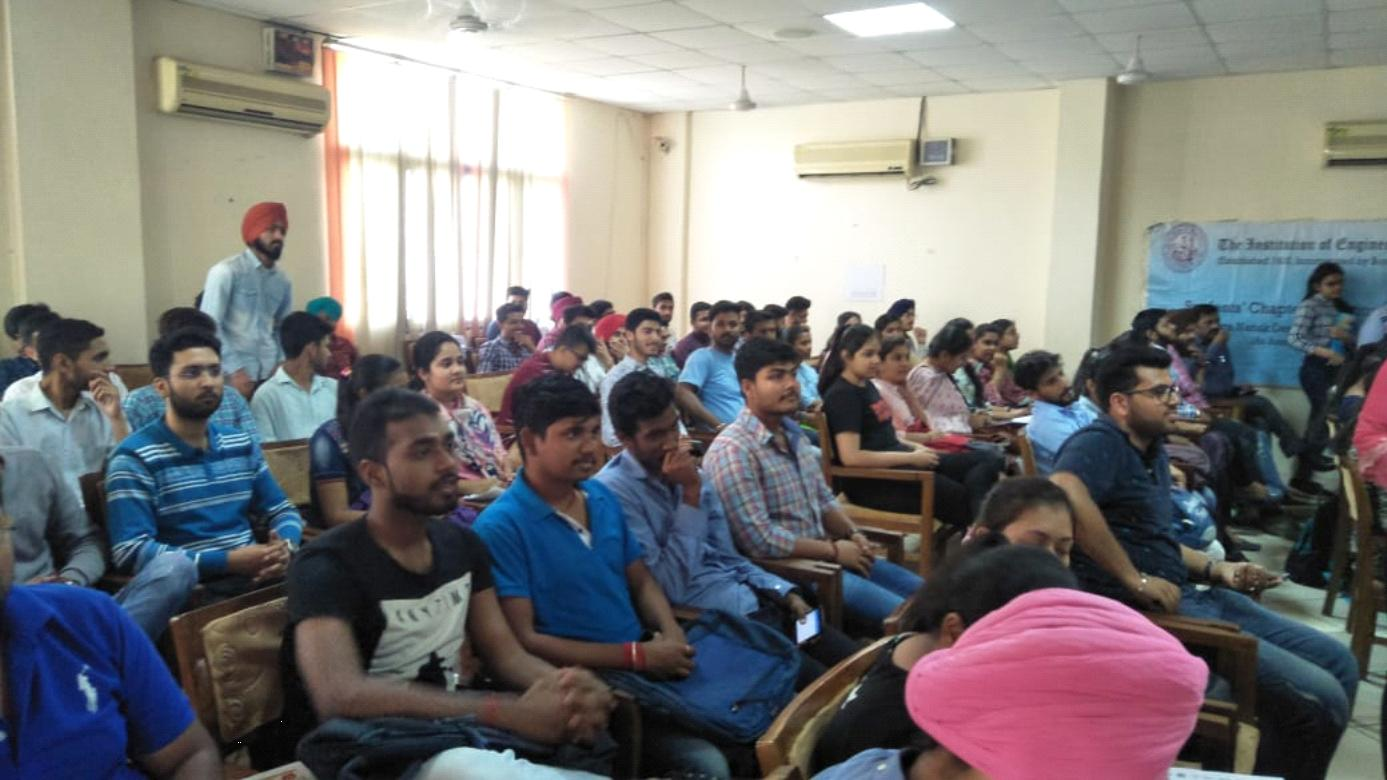
\includegraphics[width=\linewidth]{image2.jpg}
  %\caption{A boat.}
  %\label{fig:boat1}
\end{multicols}

\begin{multicols}{2}

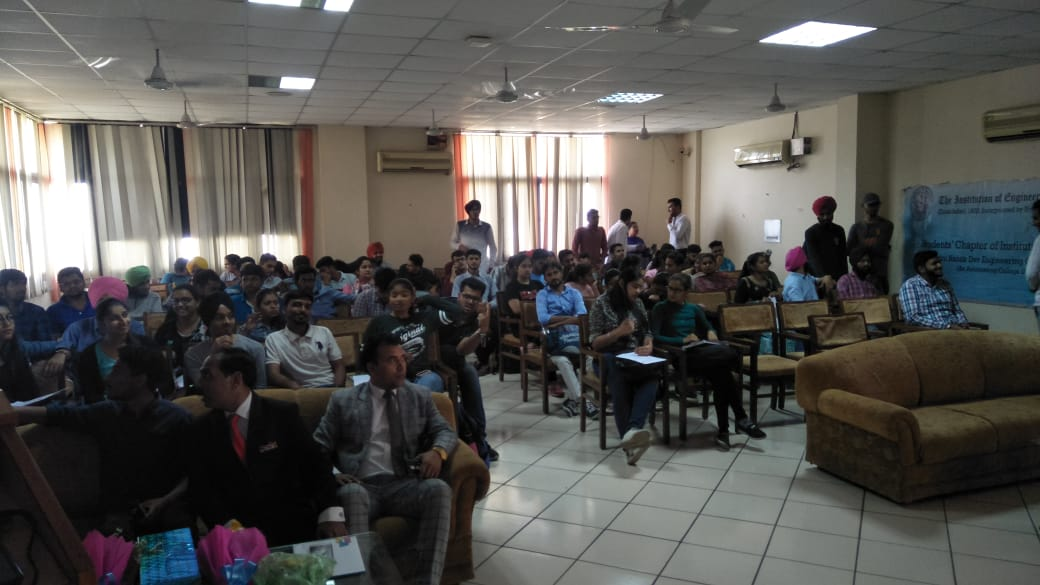
\includegraphics[width=\linewidth]{image7.jpeg}

\columnbreak
This seminar was organised to guide the students about the entrepreneurship ideas.
\end{multicols}

\newpage 

\tikz[remember picture,overlay] \node[opacity=0.8,inner sep=0pt] at (current page.center){
\includegraphics[width=\paperwidth,height=\paperheight]{5TRrp44jc.png}};
%\tikz[remember picture,overlay] \node[opacity=0.8,inner sep=0pt] at (current page.center){\includegraphics[width=\paperwidth,height=\paperheight]{md_5b0912b7c0870.png}};

\begin{multicols}{2}
This entrepreneurship awareness seminar was conducted by TEAM DYNAMIC,MILIFESTYLE MARKETING GLOBAL PRIVATE LIMITED.
\columnbreak

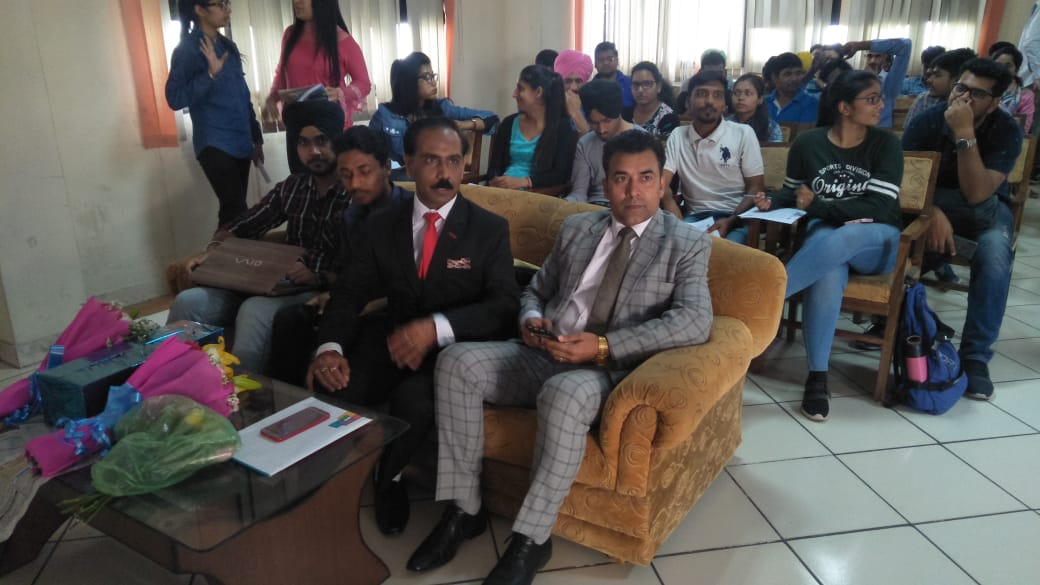
\includegraphics[width=\linewidth]{image6.jpeg}
  
\end{multicols}

\begin{multicols}{2}
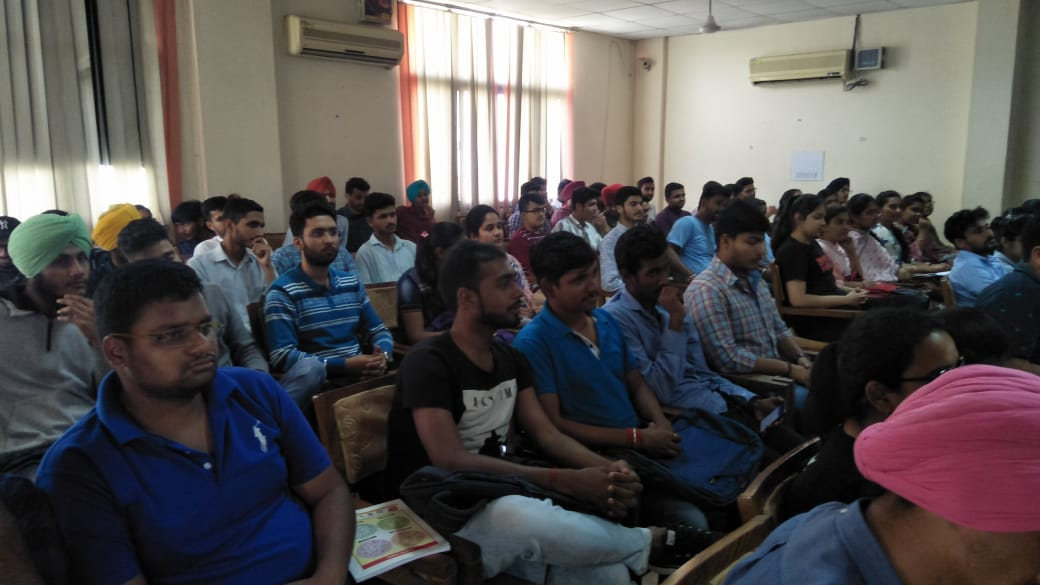
\includegraphics[width=\linewidth]{image5.jpeg}

\columnbreak
The seminar was quite interactive.
  
\end{multicols} 

%\begin{multicols}{2}
The EXPERTS had selected thirteen students from our college randomly to give their EXPERT advice to them. Overall it was very interesting.

%\columnbreak
%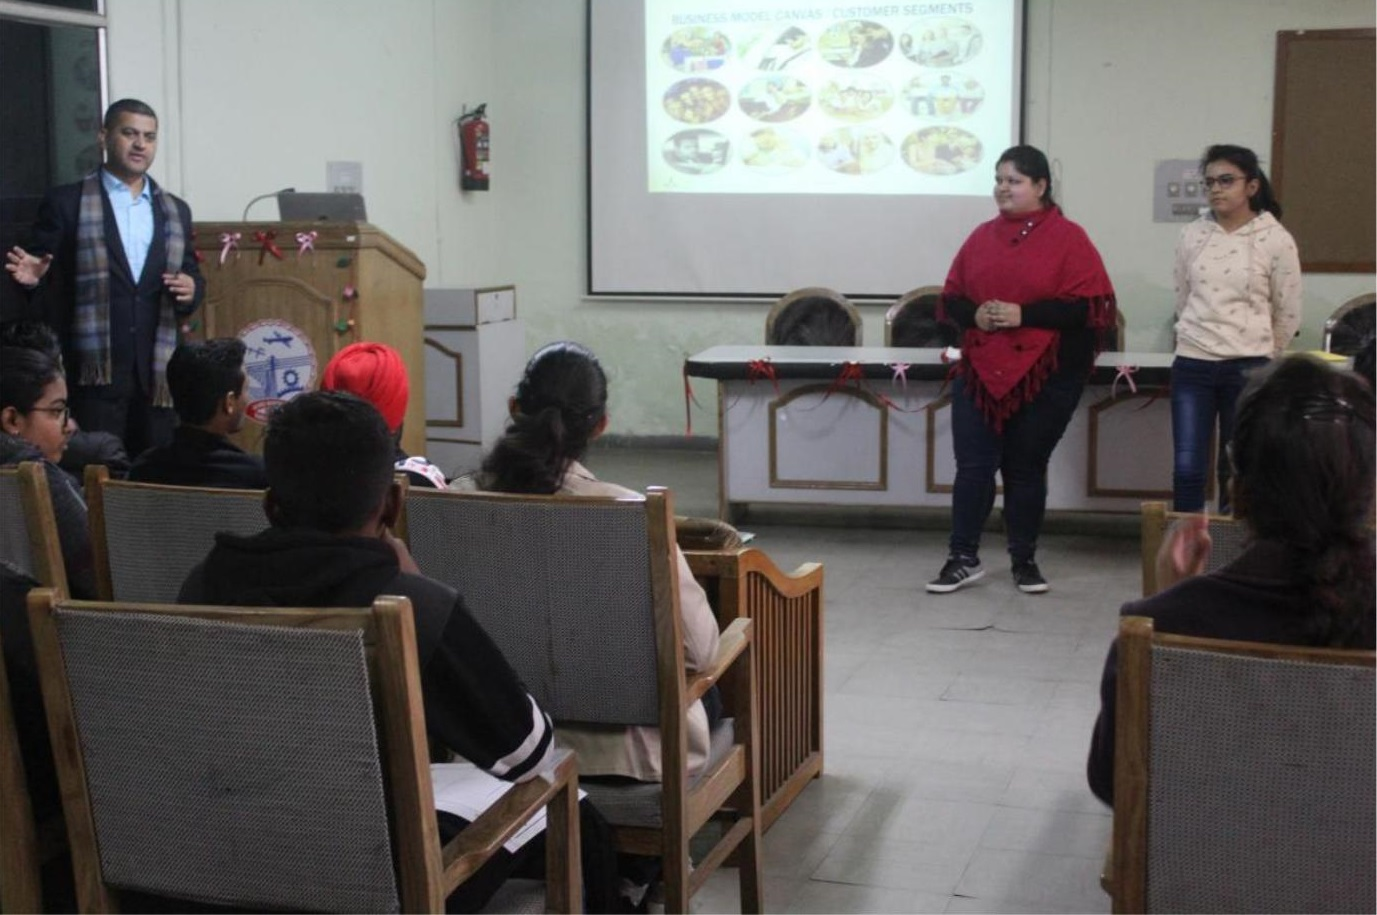
\includegraphics[width=\linewidth]{image8.jpg}
  
%\end{multicols} 

%\begin{multicols}{2}
%\includegraphics[width=\linewidth]{placeholder.jpg}

%\columnbreak
%Some paragraph
  
%\end{multicols} 

\end{Large} 
\end{center}

\newpage 

\tikz[remember picture,overlay] \node[opacity=0.8, inner sep=0pt] at (current page.center){
\includegraphics[width=\paperwidth,height=\paperheight]{5TRrp44jc.png}};
%\tikz[remember picture,overlay] \node[opacity=0.8,inner sep=0pt] at (current page.center){\includegraphics[width=\paperwidth,height=\paperheight]{md_5b0912b7c0870.png}};

\begin{center}
\Huge Pictures Section

\medskip

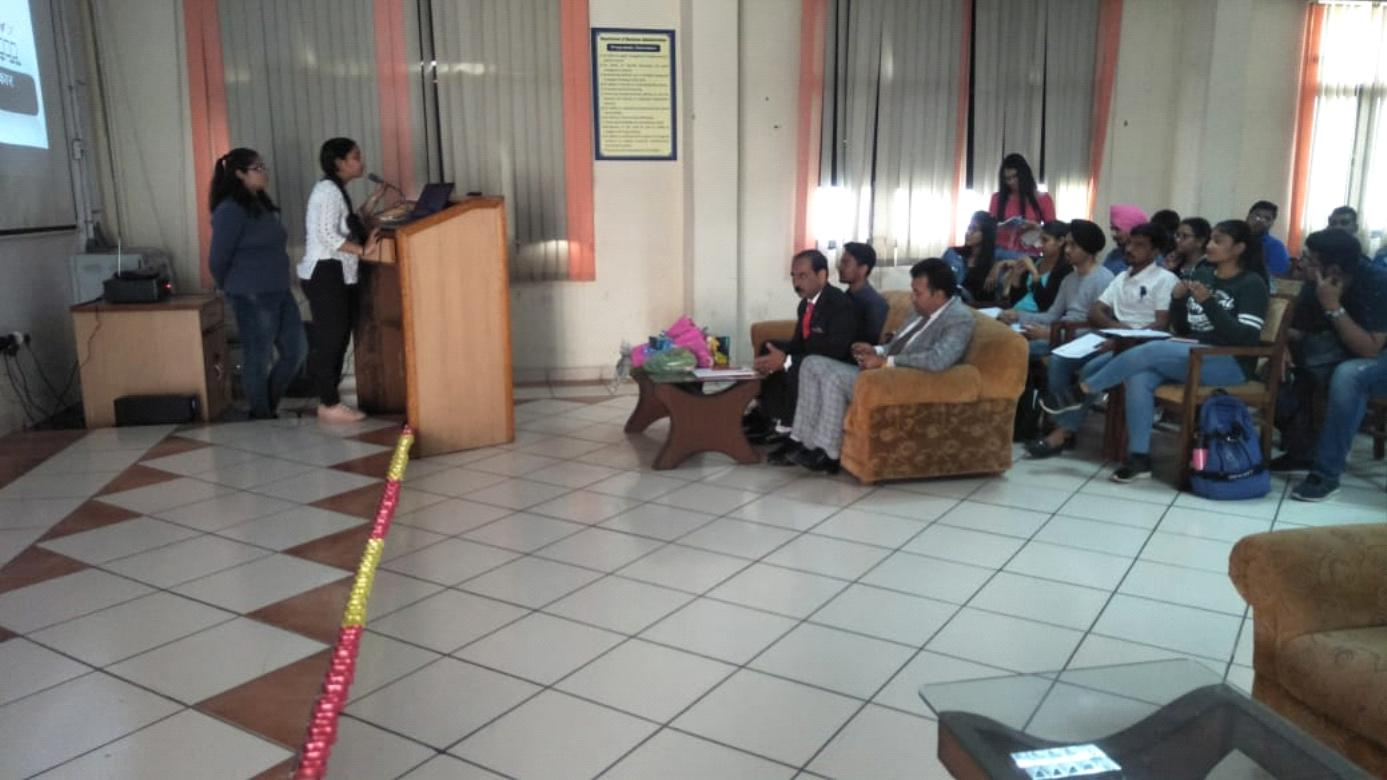
\includegraphics[height=6cm]{image1.jpg}

\medskip

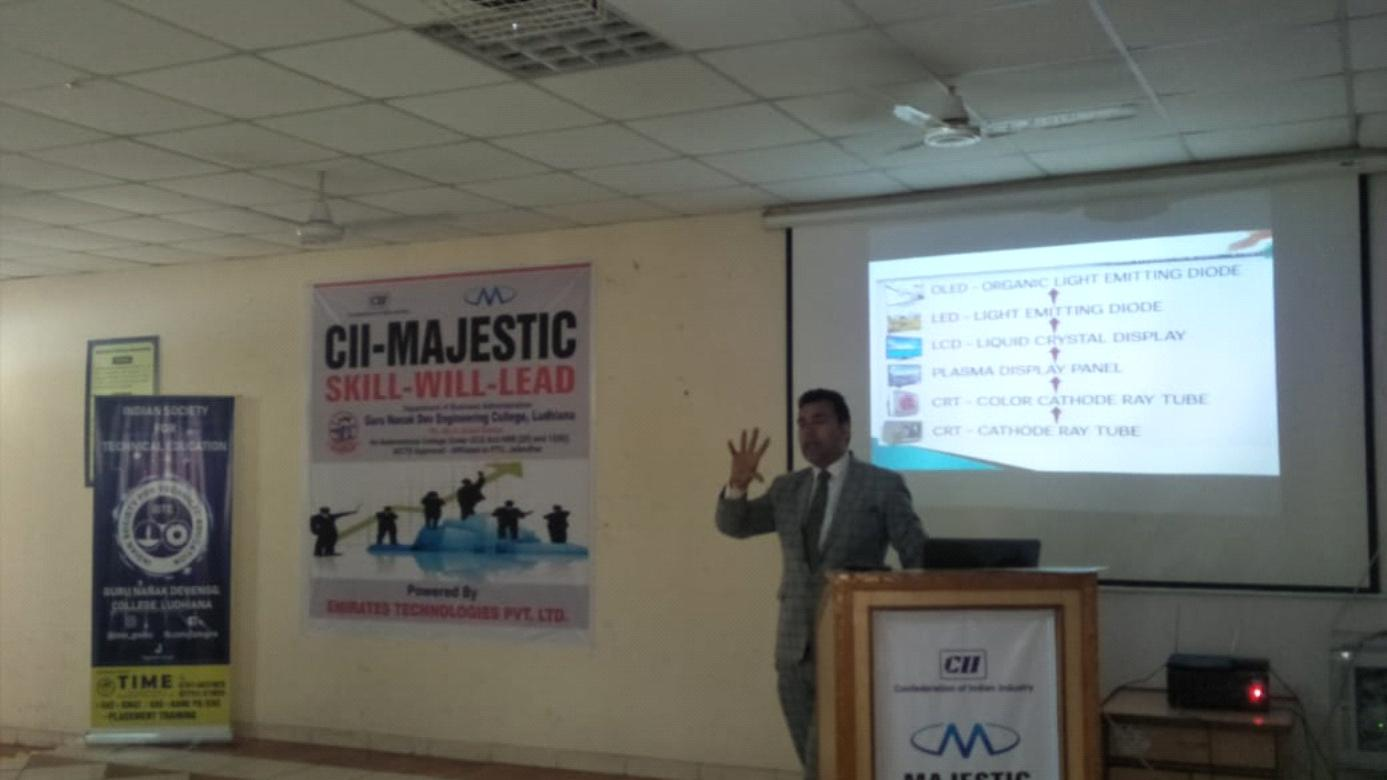
\includegraphics[height=6cm]{image3.jpg}

\medskip

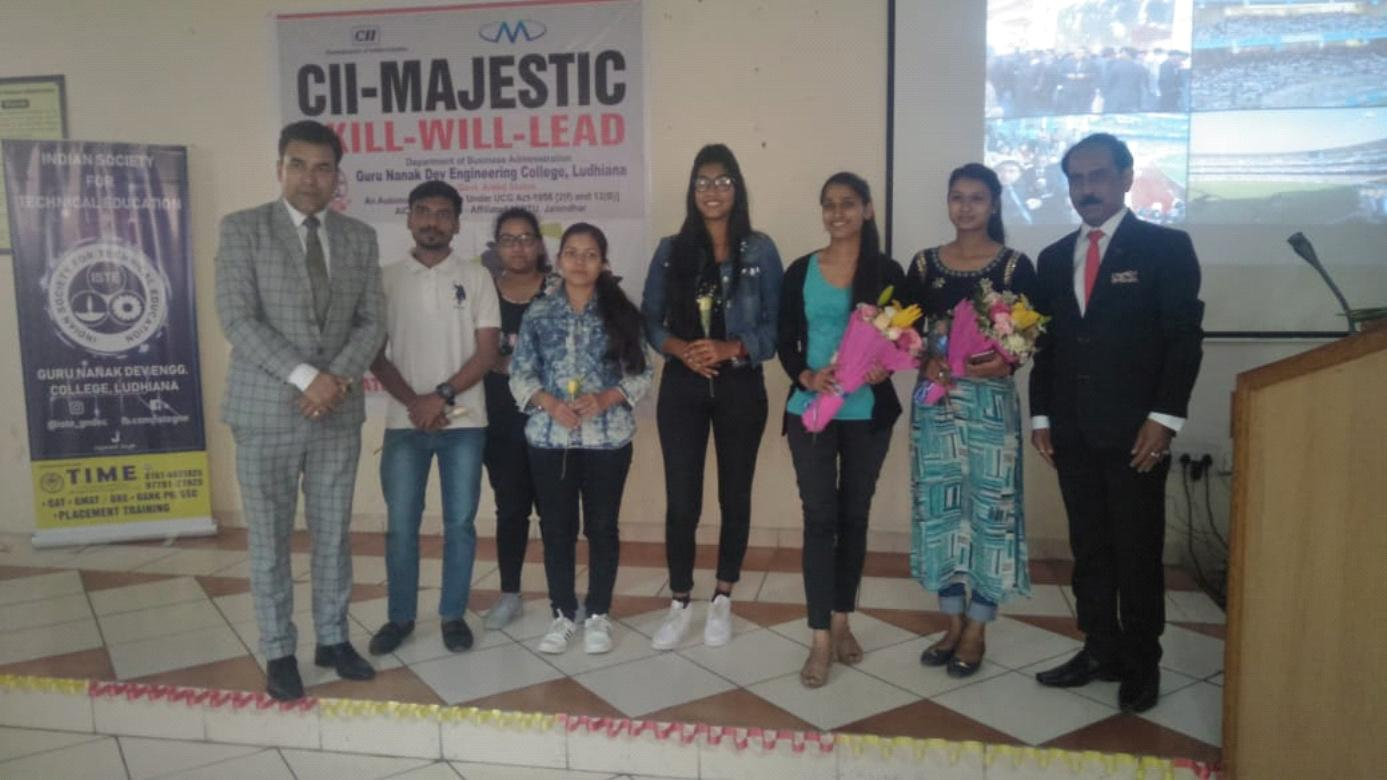
\includegraphics[height=6cm]{image4.jpg}

\end{center}

\newpage

\tikz[remember picture,overlay] \node[opacity=0.8,inner sep=0pt] at (current page.center){
\includegraphics[width=\paperwidth,height=\paperheight]{5TRrp44jc.png}};

\begin{center}
\huge Organisers list
\end{center}

\begin{table}[h!]
  \begin{center}
    \begin{tabular}{|c|c|c|c|c|c|} 
    \toprule % <-- Toprule here
      \textbf{S.No.} & \textbf{Name} & \textbf{Branch/Year} & \textbf{U.R.N} \\
      \midrule % <-- Midrule here
      1	& Kartika	       & D1 CSE	& 1805192 \\
      2 & Saloni	       & D1 CSE	& 1805985 \\
      3	& Pawan	           & D1 ECE	& 1805429 \\
      4	& Rajnish Raj	   & D1 CSE	& 1805983 \\
      5	& Ujjwaldeep Singh & D1 CE	& 1807122 \\
      6	& Amrit Kaur	   & D2 ECE	& 1706705 \\
      7	& Kanishka	       & D1 IT	& 1816050 \\
      8	& Shivam Jindal	   & D2 CSE	& 1706514 \\

      \bottomrule % <-- Bottomrule here
    \end{tabular}
  \end{center}
\end{table}

\newpage

%\tikz[remember picture,overlay] \node[opacity=0.8,inner sep=0pt] at (current page.center){
\includegraphics[width=\paperwidth,height=\paperheight]{5TRrp44jc.png}};
%\tikz[remember picture,overlay] \node[opacity=0.8,inner sep=0pt] at (current page.center){\includegraphics[width=\paperwidth,height=\paperheight]{md_5b0912b7c0870.png}};


\end{document}